\newpage
{\bfseries МРНТИ 52.47.15}

\sectionwithauthors{Н.А. Бесбаева, Г.Ж.Бимбетова, Г.М.Эфендиев, К.С. Надиров, Н.Ш.Отарбаев}{ПОЛИМЕРНЫЙ РЕАГЕНТ ДЛЯ СНИЖЕНИЯ ПОГЛОЩЕНИЯ БУРОВОГО РАСТВОРА ПРИ
БУРЕНИИ НЕФТЕГАЗОВЫХ СКВАЖИН}

\begin{center}
{\bfseries \textsuperscript{1}Н.А. Бесбаева, \textsuperscript{1}Г.Ж.Бимбетова\textsuperscript{🖂}, \textsuperscript{2}Г.М.Эфендиев, \textsuperscript{1}К.С. Надиров, \textsuperscript{1}Н.Ш.Отарбаев}

Южно-Казахстанский университет им. М. Ауэзова, Шымкент, Казахстан,

\textsuperscript{2}Институт нефти и газа, Баку, Азербайджан,

{\bfseries \textsuperscript{🖂}} Корреспондент-автор: gulmnaz@mail.ru
\end{center}

Поглощение раствора при бурении нефтяных и газовых скважин является
одним из самых распространенных осложнений, возникающих в процессе,
которое может стать причиной существенного увеличения затрат времени.
Целью данной работы явилось создание условий для снижения скорости
поглощения бурового раствора при бурении нефтегазовых скважин.
Облегченная буровая, промывочная жидкость была получена путем добавления
в рецептуру глинистого раствора полимерных реагентов, модифицированных
омыленными гудронами вакуумной дистилляции жирных кислот хлопкового
масла. Приведены результаты структурных исследований полимерного
реагента, полиакриламида, модифицированного хлопковым гудроном на
основании данных ИК-спектроскопии. По результатам полученных
спектральных характеристик полимерных композиций сделано предположение о
строении образовавшегося комплекса, обладающего набухающими свойствами,
что снижает скорость проникновения в поры пустых пород, и тем самым
способствует «уходу» раствора в затрубное пространство скважины.

Авторами сделан вывод о том, что омыленный хлопковый гудрон является
ценным сырьем для получения модифицированного полимерного реагента,
полиакриламида. На основании спектральных характеристик сделано
предположение о строении образовавшегося комплекса, обладающего сильным
набуханием при проникновений в пустых пород. Сделано предположение о
том, что полученный композиционный полимерглинистый раствор может быть
использован для снижения скорости поглощения бурового раствора при
бурении нефтегазовых скважин.

{\bfseries Ключевые слова:} нефть, буровой раствор, хлопковый гудрон,
полиакриламид, каустическая сода, поглащения раствора, снижение
поглащении, ИК-спектроскопия.

\begin{center}
{\large\bfseries МҰНАЙГАЗ ҰҢҒЫМАЛАРЫН БҰРҒЫЛАУ КЕЗІНДЕГІ БҰРҒЫЛАУ ЕРІТІНДІСІНІҢ
СІҢІРІЛУІН ТӨМЕНДЕТУГЕ АРНАЛҒАН ПОЛИМЕРЛІК РЕАГЕНТ}

{\bfseries \textsuperscript{1}Н.А.Бесбаева},
{\bfseries \textsuperscript{1}Г.Ж.Бимбетова\textsuperscript{🖂},
\textsuperscript{2}Г.М.Эфендиев, \textsuperscript{1}К.С.Надиров,
\textsuperscript{1}Н.Ш.Отарбаев}

\textsuperscript{1}М.Әуезов атындағы Оңтүстік Қазақстан университеті,
Шымкент, Қазақстан.

\textsuperscript{2} Мұнай және газ институты, Баку, Әзербайжан,

e-mail: gulmnaz@mail.ru
\end{center}

Мұнай мен газ ұңғымаларын бұрғылау кезінде ерітіндінің сіңірілуі
процесте туындайтын ең көп таралған қиындықтардың бірі, бұл уақыт
шығындарының едәуір артуына әкелуі мүмкін. Бұл жұмыстың мақсаты мұнайгаз
ұңғымаларын бұрғылау кезінде бұрғылау ерітіндінің сіңірілу жылдамдығын
төмендетуге жағдай жасау болып табылады. Жеңіл бұрғылау, шаю ерітіндісі
мақта майының май қышқылдарын вакуумдық дистилляциялау арқылы
сабындалған гудрондармен модификацияланған полимерлі реагенттердің сазды
ерітіндісін қосу арқылы алынды. ИҚ- спектроскопияның деректері негізінде
мақта гудронымен модификацияланған полимерлі реагент полиакриламидтің
құрылымдық зерттеулерінің нәтижелері келтірілген. Полимерлі
композициялардың алынған спектрлік сипаттамаларының нәтижелері бойынша
ісіну қасиеттері бар қалыптасқан кешеннің құрылымы туралы болжам
жасалды, бұл бос тау жыныстарының кеуектеріне ену жылдамдығын
төмендетеді және осылайша ерітіндінің ұңғыманың құбырлы кеңістігіне
"кетуіне" ықпал етеді.

Авторлар сабындалған мақта гудроны модификацияланған полимерлі реагент,
полиакриламид алу үшін құнды шикізат болып табылады деген қорытындыға
келді. Спектрлік сипаттамаларға сүйене отырып, бос тау жыныстарына ену
кезінде қатты ісінуі бар қалыптасқан кешеннің құрылымы туралы болжам
жасалады. Алынған композициялық полимерсазды ерітіндісі мұнайгаз
ұңғымаларын бұрғылау кезінде бұрғылау ерітіндісінің сіңірілу жылдамдығын
төмендету үшін қолдануға болады деген болжам жасалды.

{\bfseries Түйін сөздер:} мұнай, бұрғылау ерітіндісі, мақта гудроны,
полиакриламид, каустикалық сода, ерітіндіні сіңіру, сіңіруді азайту, ИҚ
спектроскопиясы.

\begin{center}
{\large\bfseries POLYMER REAGENTS TO REDUCE THE ABSORPTION OF DRILLING MUD DURING
DRILLING OF OIL AND GAS WELLS}

{\bfseries \textsuperscript{1}N.A. Besbaeva},
{\bfseries \textsuperscript{1}G.ZH. Bimbetova\textsuperscript{🖂},
\textsuperscript{2}G.M. Afandiyev, \textsuperscript{1}K.S. Nadirov},
{\bfseries \textsuperscript{1}N.Sh.Otarbaev}

\textsuperscript{1}M. Auezov South Kazakhstan State University,
Shymkent, Kazakhstan,

\textsuperscript{2}Institute of Oil and Gas, Baku, Azerbaijan,

e-mail: gulmnaz@mail.ru
\end{center}

The absorption of the solution during drilling of oil and gas wells is
one of the most common complications that arise in the process, which
can cause a significant increase in time spent. The purpose of this work
was to create conditions for reducing the rate of absorption of drilling
mud during drilling of oil and gas wells. A lightweight drilling and
washing liquid was obtained by adding polymer reagents modified with
saponified tar from vacuum distillation of fatty acids of cottonseed oil
to the clay solution formulation. The results of structural studies of a
polymer reagent, polyacrylamide modified with cotton tar, based on IR
spectroscopy data are presented. Based on the results of the obtained
spectral characteristics of polymer compositions, an assumption is made
about the structure of the formed complex, which has swelling
properties, which reduces the rate of penetration into the pores of
empty rocks, and thereby contributes to the "withdrawal" of the solution
into the annulus of the well.

The authors concluded that saponified cotton tar is a valuable raw
material for the production of a modified polymer reagent,
polyacrylamide. Based on the spectral characteristics, an assumption is
made about the structure of the formed complex, which has a strong
swelling during penetration into empty rocks. It is assumed that the
resulting composite polymer clay solution can be used to reduce the
absorption rate of drilling mud during drilling of oil and gas wells.

{\bfseries Keywords:} oil; drilling mud, cotton tar; polyacrylamide,
caustic soda, solution absorption, reduced absorption, IR spectroscopy.

\begin{multicols}{2}
{\bfseries Введение.} Бурение нефтегазовых скважин часто сопровождаются
возникновением аварий и осложнений, ликвидация которых требует
определенного времени и значительных материальных затрат для буровых
компаний. Осложнения, связанные с поглощением бурового раствора при
вскрытии и освоении продуктивных горизонтов в процессе бурения
нефтегазовых скважин, являются главными причинами отклонения от сроков
освоения скважины, предусмотренных геолого-техническим нарядом. Это, в
частности, наблюдается при бурении скважин на месторождениях Южно -
Торгайской впадины, где почва является рыхлой со сложными геологическими
свойствами с содержанием значительного количества минеральных солей
{[}1-4{]}.

Необходимо отметить, что в целом гелогические особенности
Южно-Торгайского осадочного бассейна сегодня в достаточной степени
изучены геолого-геофизическими методами. В настоящее время на этих
месторождениях наблюдается тенденция к~истощению запасов длительно
разрабатываемых месторождений, и, следовательно, источником прироста
запасов углеводородов становится поиск и разведочное бурение новых
нефтяных и газовых скважин. Несмотря на то, что начиная со второй
половины прошлого столетия, успешно эксплуатируются известные
месторождения: Карабулак, Кумколь, Сарыбулак, Южный Сарыбулак,
Южно-Арысское, Ащысай, Акшабулак, Кенлик, Коныс и другие, все они
эксплуатируются в условиях большой обводненности. Нефти этих
месторождений являются высокопарафинистыми, малосернистыми и практически
все эмульсионные {[}5{]}.

Для проведения работ по строительству для бурения разведочных,
эксплуатационных и других скважин, необходимы буровые промывочные
растворы с расширеннными функциональными свойствами. На сегодня
актуальной является проблема объемов снижения поглощения бурового
раствора в процессе бурения нефтегазовых скважин в сложных геолгических
условиях. По мнению авторов комплексное решение этих задач, будет
способствовать снижению затрат на сокращение сроков и стоимости процесса
бурения эксплуатационных скважин.

Система «Скважина -- пласт» является сообщающимся сосудом. Напомним, что
поглощение это процесс частичной или практически полного ухода буровой,
промывочной жидкдости при бурении в пласт, что сопровождается постоянным
снижением его объемов в емкостях циркуляционной ситемы. Причинами потери
бурового раствора при его циркуляции являются превышение давления столба
жидкости в скважине над пластовым давлением. Следовательно, чем больше
разница в давлении, тем больше поглощение и потери раствора в системе. В
настоящее время в практике бурильных работ используют буровые растворы
на водной основе, которые состоят из дисперсной среды -- воды,
дисперсной фазы -- твердой, либо эмульгированной и различных
водорастворимых электролитов, полиэлектролитов, щелочей, кислот,
ионогенных и неионогенных поверхностно-активных веществ. В качестве
твердой фазы в буровом растворе используется активная составляющая --
глина и различные химические реагенты. Эмульгированной фазой может быть
нерастворимая в воде жидкость, например нефть, масла и другие
компоненты.

При этом различают 3 категории интенсивности поглощений бурового
раствора: малой интенсивности (до 10-15 м\textsuperscript{3}/ч), средней
интенсивности (до 40-60 м\textsuperscript{3}/ч) и высокой интенсивности
(более 60 м\textsuperscript{3}/ч).

Поглощение бурового раствора объясняется наличием пор, трещин и пустот в
породе, а также ее недостаточной устойчивостью перед давлением жидкости
в скважине, в результате чего возникает гидроразрыв пласта.

Определение интенсивности поглощения производится с использованием
различных методик, так например, оценка соотношения количества
закачиваемого в скважину раствора и объема его поступления из скважины в
приемную емкость {[}6{]}.

В связи с этим одним из направлений повышения эффективности
строительства скважин является совершенствование составов буровых
растворов за счет применения полимерных реагентов, в том числе
биополимеров, которые продуцируются микробными культурами на углеводах.
Биополимеры обладают комплексом уникальных свойств, основным из которых
является возможность эффективного управления реологической
характеристикой бурового раствора за счет их псевдопластичности, которая
обеспечивает очистку скважин от выбуренной породы при низких
гидродинамических сопротивлениях {[}7{]}.~

В работах авторов {[}8-11{]} показано, что значительный эффект повышения
технико-экономических показателей бурения достигается применением
безглинистых и малоглинистых облегченных растворов.

Для регулирования свойств малоглинистых растворов применяют глинопорошки
различных сортов, обычно 5-10\%, с добавлением смол и полимеров
{[}12{]}. Полимеры в составе бурового раствора для бурения скважин
выполняют следующие функции:~укрепление стенок скважины и её
очистка;~уменьшение износа инструмента и защита его от
коррозии;~регулирование вязкости и плотности раствора. В практике
бурения скважин полиакриламид используется как стабилизатор, эффективный
понизитель фильтрации глинистых буровых растворов. Надо сказать, что
полиакриламид марки АК-636 выполняет функцию понижения фильтрации только
в глинистых буровых растворах и наоборот, как понизитель фильтрации в
растворах без твердой фазы проявляет небольшую активность. Однако в
качестве загустителя водной фазы может с успехом использоваться в
безглинистых системах, в том числе, в минерализованных водных растворах.

Эффективными мерами борьбы с проблемой поглощения бурового раствора
является его предупреждение. Растворы с высокими реологическими и
механическими свойствами менее интенсивно ухо­дят в пласт. При этом
решающее значение имеет дифференциаль­ное давление в системе «скважина --
пласт». Предотвращаю­щие уход жидкости в пласт можно предупредить
следующими мерами: 1) Снижение дифференциального давления; 2) Повышение
реологических свойств раствора; 3) Уменьшение расхода жидкости при
циркуляции; 4) Применение облегченных растворов, газообразных агентов,
аэрированной жидкости; 5) Применение наполнителей; 6) Промежуточная
промывка; 7) Предупреждение сальникообразования на долоте и утяжеленных
бурильных труб (УБТ)\textsc{;} 8) Соответствующая компоновка нижней
части бурильной колонны~(КНБК), позволяющей увели­чить зазоры кольцевого
пространства; 9) Употребление комовой глины или глин грубого помола для
приготовления бурового раствора {[}6{]}.

Катастрофические уходы жидкости в пласт (более 60
м\textsuperscript{3}/ч) ликвидируются тампонированием поровых каналов
(трещин) специальными веще­ствами. Это может быть достигнуто тампонажным
цементом, или его смесью с другими материалами (бентонит, гипс,
алебастр, асбест, древес­ные опилки и др.).

Однако, известно, что основные потери бурового раствора происходят в
зоне работы породоразрущающегося инструмента (долота) обсадной колонны.
Это происходит на глубине скважины, чем рыхлее корка стенки скважины,
тем больше будет боковой отток буровой промывочной жидкости в заколонное
пространство через пористую породу.

Целью данной работы являлась снижение скорости поглощения бурового
раствора при бурении нефтегазовых скважин путем добавления в рецептуру
глинистого раствора полимерного реагента полиакриламида,
модифицированного омыленным гудроном дистилляции жирных кислот масла
хлопчатника.

{\bfseries Материалы и методы.} Основным ингредиентом глинистого бурового
раствора является~бентонит. Натуральный глинистый минерал (глинопорошок)
при насыщении его водой разбухает примерно в 15 раз. Так образуется
гелевая масса --- плотная и скользкая. Местный бентонит месторождения
Дарбаза (Туркестанская область) является более подходящей
структурообразующей добавкой к буровой промывочной жидкости, так как ее
свойства улучшаются с модифицированными полимерными добавками.

Исследование фильтрационных свойств горных породы с целью определения
скорости поглащения бурового раствора проводилось на лабораторной
установке УИК-С(2) на образцах горных пород (керна), при соотношении
компонентов раствора в рецептуре, указанной ниже. Состав глинистого
раствора, \%: бентонит -9-10; полиакриламид -- 6-7; омыленный хлопковый
гудрон -- 4-5; мел (СаСО\textsubscript{3}) - 5-6; КМЦ-ТС -- 0,8-1,0;
сода кальцинированная (Nа\textsubscript{2}СО\textsubscript{3}) - 0,1-0,2
и вода-остальное.

В данной работе были получены малоглинистые растворы с добавлением
полиакриламида, модифицированного омыленным хлопковым гудроном. Омыления
гудрона осуществлялась 20\% раствором гидроксида натрия при температуре
110\textsuperscript{о}С. Полимерный раствор при циркуляции в составе
бурового раствора проникает в поры, трещины и пустоты породы, которая
является недостаточно устойчивой при рабочем давлении жидкости в
скважине.

{\bfseries Результаты и обсуждение.} Приведены результаты структурных
исследований полимерного реагента с применением ИК-спектроскопии. На
рисунке 1 представлены ИК-спектры модифицированного полимерного
реагента, полученные на приборе ИК-Фурье спектрометр Shimadzu IR
Prestige - 21 с приставкой нарушенного полного внутреннего отражения
(НПВО) Miracle фирмы PikeTechnologies.
\end{multicols}

\begin{figure}[H]
	\centering
	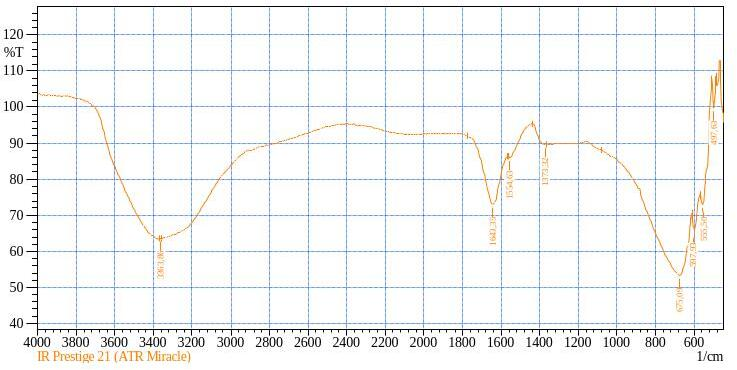
\includegraphics[width=0.8\textwidth]{assets/1262}
	\caption*{Рис. 1 - ИК-спектры модифицированного полимерного реагента}
\end{figure}

\begin{multicols}{2}
Результаты ИК-спектроскопических исследований модифицированного
полимерного реагента показывают, что полосы поглощения с пиками
интенсивностью 3364-3356 см\textsuperscript{-1}, которые можно отнести к
валентным (ν) колебаниям O--Н связи в группах, являются характерными для
модифицированного полиакриламида.

Менее интенсивные полосы частотой 1643-1566 см-\textsuperscript{1} можно
отнести к валентным колебаниям карбонильных групп нафталинового ядра
молекулы госсипола, которые в условиях получения гудрона образуется при
окислении альдегидных групп. Полосы при 1554 -- 1439
см\textsuperscript{-1}, можно отнести к валентным колебаниям
ароматических колец госсипола. Полосы поглощения с пиками 1373-1365
см\textsuperscript{-1} можно отнести к валентным (сл.) колебаниям
проявляющиеся в спектрах функциональных групп жирных кислот. Сильный пик
в области 675--617 см\textsuperscript{-1} можно отнести внеплоскостным
деформационным колебаниям С-Н.

Таким образом результаты ИК-спектроскопии указывает на изменение
структуры полученного модифицированного полимерного реагента, который
может быть использован добавкой к буровой, промывочной жидкости с целью
снижение объема его потерь при бурении скважин на нефть и газ.
\end{multicols}

\begin{figure}[H]
	\centering
	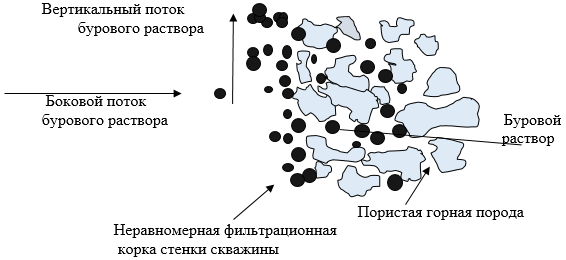
\includegraphics[width=0.9\textwidth]{assets/1262.1}
	\caption*{Рис. 2 - Схема, показывающая «уход» бурового раствора через горную породу}
\end{figure}

\begin{figure}[H]
	\centering
	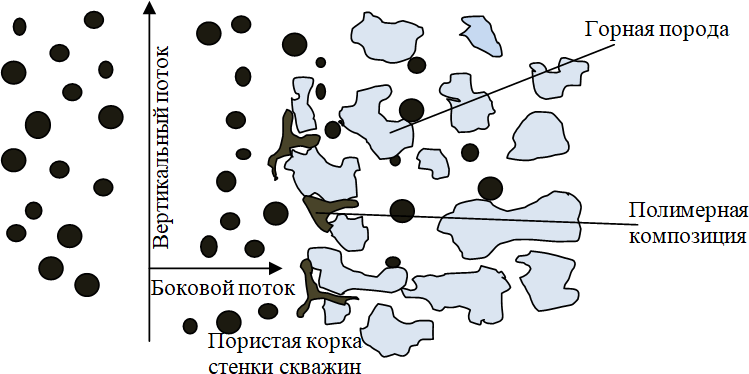
\includegraphics[width=0.8\textwidth]{assets/1263}
	\caption*{Рис. 3 - Схема снижения скорости поглощения бурового раствора путем введения полимерной композиции}
\end{figure}

\begin{multicols}{2}
На рисунках 2 и 3 представлены результаты экспериментальных данных по
изменению скорости поглощения бурового раствора без добавления (рисунок
2) и в присутствии модифицированного полимерного реагента (рисунок 3).
Из данных рисунков видно, что в первом случае наблюдается уход бурового
раствора через трещины и пустоты горной породы, тогда как во втором
случае макромолекулы модифицированного полимерного реагента набухают и
препятствуют проникновению раствора через породы, которые были
определены по методике изменения объема от оторочки раствора полимера
{[}13{]}.~

Таким образом, показано, что раствор при прохождении в пористую породу
(боковой поток) из-за содержащегося в нем полимерного композита снижает
поток раствора через корковый слой, в результате чего снижается
поглощение раствора. Полимерная композиция вначале набухает, затем в
пористой среде предотвращает или снижает скорость поглощения буровой
промывочной жидкости (рисунок 3).

Предварительный расчет показывает что эффект снижения степени поглощения
от использования полимерной композиции составляет 12,5\%.

Таким образом, полученные данные показывают, что полученная авторами
полимерная композиция на основе полиакриламида и хлопкового гудрона
частично проникает в пространство между горной породой и закупоривает ее
за счет смолообразной массы. На основании экспериментальных данных
показано, что омыленный гудрон является ценным сырьем для получения
модифицированных полимерных реагентов по снижению поглощения бурового
раствора при бурении нефтегазовых скважин.

{\bfseries Выводы.} Авторами сделан вывод о том, что омыленный хлопковый
гудрон является ценным сырьем для получения модифицированного
полимерного реагента на основе полиакриламида. На основании спектральных
характеристик сделано предположение о строении образовавшегося
комплекса, обладающего сильными набухающими свойствами, который
способстует предотвращению проникновения бурового раствора в
пространство пустых горных пород. Сделано предположение о том, что
полученный композиционный полимерглинистый раствор может быть
использован для снижения скорости поглощения бурового раствора при
бурении нефтегазовых скважин.
\end{multicols}

\begin{center}
{\bfseries Литература}
\end{center}

\begin{noparindent}
1.
  Надиров К.С., Сакибаева С.А., БимбетоваГ.Ж. Поверхностно-активные
  вещества на основе госсиполовой смолы и их использование. - Шымкент:
  Южно-Казахстанский государственный университет им. М.Ауэзова, 2013. -
  230 с.

2.
  Пат. №27482 Республика Казахсатн МПК С09К 8/34 (2006.01)
  Модифицированный буровой раствор. / Надиров К.С., Бондаренко В.П.,
  Голубев В.Г. БимбетоваГ.Ж., Надирова Ж.К., Садырбаева А.С., Орымбетова
  Г.Э., Ибрагимов Ф.Р., Джусенов А.У.; заявитель и патентообладатель
  ЮжноКазахстанский государственный университет им. М. Ауезова.
  -№2012/1022.1; заявл. 05.10.2012; опубл. 15.10.2013. Бюл. №10.

3.
  Бондаренко В.П., Исатаев А.А., Р. Мустафина. Исследования свойств
  жидкостей для глушения скважин//Труды Международной
  научно-практической конференции «Ауэзовские чтения -11: Казахстан на
  пути к обществу знаний: инновационные направления развития науки,
  образования и культуры», посвященной 115-летнему юбилею М. Ауэзова.
  Шымкент. - 2012. -С.40-44.

4.
  Голубев В.Г., Надиров К.С., Бондаренко В.П., Жантасов М.К., Джусенов
  А.У. Исследование влияния температуры на термостойкость, фильтроотдачу
  и эффективную вязкость гидрофобно-эмульсионных растворов // Труды
  Международной научно-практической конференции «Развитие науки,
  образования и культуры независимого Казахстана в условиях глобальных
  вызовов современности», посвященной 70-летию Южно-Казахстанского
  Государственного университета им. М. Ауэзова. Шымкент. - 2013. -Т. 4.
  - С.11-14.

5.
  Надиров Н.К. Высоковязкие нефти и природные битумы: в 5 т:
  История.Бассейны. Свойства. -Алматы: «Ғылым», 2001. - Т.1. -360 с.

6.
  Умедов Ш. Х.Разработка эффективных составов промывочных жидкостей для
  борьбы с осложнениями при бурении нефтяных и газовых скважин: дис.
  \ldots{} док. тех. наук 05.15.10 -- Технология бурения и освоения
  скважин.

7.
  Рахимов А.А., Рахимов Э.А., Курбанов А.Н., Умедов Ш.Х. Снижение
  гидродинамического давления при циркуляции бурового раствора //
  Узбекский журнал нефти и газа. -- Ташкент, 1999. - № 1. -- С. 20 - 24.

8.
  Кадыров Н.А., Норкулова К.Т., Надиров К.С. Технология получения
  бурового реагента на основе масложировых и химических отходов
  производства// Материалы Юбилейной международной научно-практической
  конференции «Белые -- ночи-2013». - Санкт-Петербург, 2013. - Ч.2. -
  С.107-108.

9.
  Андерсон Б.А., Бочкарев Г.П. Растворы на полимерной основе для бурения
  скважин // обзорная информация, Сер. Бурение. -- М.: ВНИИОЭНГ, 1986.
  -56с.

10.
  Ишмухамедова Н.К., Кенжебеков Н.М. Модифицированный буровой раствор//
  Нефть и газ. - 2005. - №3. - С.132-133.

11.
  Ишмухамедова Н.К., Надиров Н.К., Эфендиев Г.М. Буровой раствор на
  основе природного сырья, отходов нефтехимической и
  нефтеперерабатывающей промышленности // Вестник Атырауского института
  нефти и газа. - 2009. - № 4(19). - С.106-109.

12.
  Бондаренко В.П., Надиров К.С., Голубев В.Г., Садырбаева А.С.,
  Колесников А.С. Реагенты комплексного действия на основе
  модифицированных гудронов хлопкового масла для нефтегазовой отрасли:
  монография. - Шымкент. --Изд. ИП «Туркенич», 2017. -248 с.
\end{noparindent}

\begin{center}
{\bfseries References}
\end{center}

\begin{noparindent}
1.
  Nadirov K.S., Sakibaeva S.A., BimbetovaG.Zh. Poverkhnostno-aktivnye
  veshchestva na osnove gossipolovoi smoly i ikh
  ispol\textquotesingle zovanie. - Shymkent: Yuzhno-Kazakhstanskii
  gosudarstvennyi universitet im. M.Auezova, 2013. - 230 s. {[}in
  Russian{]}

2.
  Pat. №27482 Respublika Kazakhsatn MPK S09K 8/34 (2006.01)
  Modifitsirovannyi burovoi rastvor. / Nadirov K.S., Bondarenko V.P.,
  Golubev V.G. BimbetovaG.Zh., Nadirova Zh.K., Sadyrbaeva A.S.,
  Orymbetova G.E., Ibragimov F.R., Dzhusenov A.U.;
  zayavitel\textquotesingle{} i patentoobladatel\textquotesingle{}
  YuzhnoKazakhstanskii gosudarstvennyi universitet im. M. Auezova.
  -№2012/1022.1; zayavl. 05.10.2012; opubl. 15.10.2013. Byul. №10. {[}in
  Russian{]}

3.
  Bondarenko V.P., Isataev A.A., Mustafina R. Issledovaniya svoistv
  zhidkostei dlya glusheniya skvazhin//Trudy Mezhdunarodnoi
  nauchno-prakticheskoi konferentsii «Auezovskie chteniya -11:
  Kazakhstan na puti k obshchestvu znanii: innovatsionnye napravleniya
  razvitiya nauki, obrazovaniya i kul\textquotesingle tury»,
  posvyashchennoi 115-letnemu yubileyu M. Auezova. Shymkent. - 2012.
  -S.40-44. {[}in Russian{]}

4.
  Golubev V.G., Nadirov K.S., Bondarenko V.P., Zhantasov M.K., Dzhusenov
  A.U. Issledovanie vliyaniya temperatury na
  termostoikost\textquotesingle, fil\textquotesingle trootdachu i
  effektivnuyu vyazkost\textquotesingle{}
  gidrofobno-emul\textquotesingle sionnykh rastvorov // Trudy
  Mezhdunarodnoi nauchno-prakticheskoi konferentsii «Razvitie nauki,
  obrazovaniya i kul\textquotesingle tury nezavisimogo Kazakhstana v
  usloviyakh global\textquotesingle nykh vyzovov sovremennosti»,
  posvyashchennoi 70-letiyu Yuzhno-Kazakhstanskogo Gosudarstvennogo
  universiteta im. M. Auezova. Shymkent. - 2013. -T. 4. - S.11-14. {[}in
  Russian{]}

5.
  Nadirov N.K. Vysokovyazkie nefti i prirodnye bitumy: v 5 t:
  Istoriya.Basseiny. Svoistva. -Almaty: «Ғylym», 2001. - T.1. -360 s.
  {[}in Russian{]}

6. Umedov Sh.Kh. Razrabotka effektivnykh sostavov promyvochnykh
zhidkostei dlya bor\textquotesingle by s oslozhneniyami pri burenii
neftyanykh i gazovykh skvazhin: dis. \ldots{} dok. tekh. nauk 05.15.10
-- Tekhnologiya bureniya i osvoeniya skvazhin. {[}in Russian{]}

7. Rakhimov A.A., Rakhimov E.A., Kurbanov A.N., Umedov Sh.Kh. Snizhenie
gidrodinamicheskogo davleniya pri tsirkulyatsii burovogo rastvora //
Uzbekskii zhurnal nefti i gaza. -- Tashkent, 1999. - № 1. -- S. 20 - 24.
{[}in Russian{]}

8. Kadyrov N.A., Norkulova K.T., Nadirov K.S. Tekhnologiya polucheniya
burovogo reagenta na osnove

maslozhirovykh i khimicheskikh otkhodov
proizvodstva// Materialy Yubileinoi mezhdunarodnoi

nauchno-prakticheskoi
konferentsii «Belye -- nochi-2013». - Sankt-Peterburg, 2013. - Ch.2. -
S.107-108. {[}in Russian{]}

9. Anderson B.A., Bochkarev G.P. Rastvory na polimernoi osnove dlya
bureniya skvazhin // obzornaya informatsiya, Ser. Burenie. -- M.:
VNIIOENG, 1986. -56 s. {[}in Russian{]}

10. Ishmukhamedova N.K., Kenzhebekov N.M. Modifitsirovannyi burovoi
rastvor// Neft\textquotesingle{} i gaz. - 2005. - №3. - S.132-133. {[}in
Russian{]}

11. Ishmukhamedova N.K., Nadirov N.K., Efendiev G.M. Burovoi rastvor na
osnove prirodnogo syr\textquotesingle ya, otkhodov neftekhimicheskoi i
neftepererabatyvayushchei promyshlennosti // Vestnik Atyrauskogo
instituta nefti i gaza. - 2009. - № 4(19). - S.106-109. {[}in Russian{]}

12. Bondarenko V.P., Nadirov K.S., Golubev V.G., Sadyrbaeva A.S.,
Kolesnikov A.S. Reagenty kompleksnogo deistviya na osnove
modifitsirovannykh gudronov khlopkovogo masla dlya neftegazovoi otrasli:
monografiya. - Shymkent. --Izd. IP «Turkenich», 2017. -248 s. {[}in
Russian{]}
\end{noparindent}

\emph{{\bfseries Сведения об авторах}}

\begin{noparindent}
Бесбаева Н.А. - PhD докторант, Южно-Казахстанский университет им. М.
Ауэзова, Шымкент, Казахстан,

е-mail:besbaeva.nursulu@mail.ru;

Бимбетова Г.Ж.- кандидат технических наук, профессор, Южно-Казахстанский
университет им. М. Ауэзова, Шымкент, Казахстан, е-mail: gulmnaz@mail.ru;

Эфендиев Г.М.- доктор технических наук, профессор, Институт нефти и
газа, Баку, Азербайджан,

е-mail:galib\_2000@yahoo.com;

Надиров К.С.- доктор химических наук, профессор, Южно-Казахстанский
университет им. М. Ауэзова, Шымкент, Казахстан, е-mail:
nadirovkazim@mail.ru;

Отарбаев Н.Ш.- PhD, старший преподаватель, Южно-Казахстанский
университет им. М. Ауэзова, Шымкент, Казахстан, е-mail:
otarbaevn@mail.ru;
\end{noparindent}

\emph{{\bfseries Information about the authors}}

\begin{noparindent}
Besbaeva N.A. - PhD doctoral student, M. Auezov South Kazakhstan
University, Shymkent, Kazakhstan,

е-mail:besbaeva.nursulu@mail.ru;

Bimbetova G.Zh. - Candidate of technical Sciences, Professor, M. Auezov
South Kazakhstan University, Shymkent, Kazakhstan, е-mail:
gulmnaz@mail.ru;

Efendiev G.M. - Doctor of technical Sciences, Professor, Institute of
Oil and Gas, Baku, Azerbaijan,

е-mail:galib\_2000@yahoo.com;

Nadirov K.S. - Doctor of chemical Sciences, Professor, M. Auezov South
Kazakhstan University, Shymkent, Kazakhstan, е-mail:
nadirovkazim@mail.ru;

Otarbaev N.Sh.\textsuperscript{-} PhD, senior lecturer, M. Auezov South
Kazakhstan University, Shymkent, Kazakhstan, е-mail: otarbaevn@mail.ru
\end{noparindent}
